\chapter{Further thoughts on kinetic dominance}
\label{chap:cls}

\section{Recap}
The classical equations of motion for single field inflation are
governed by:
%
\begin{align}
  \dot{H} + H^2 
  &= - \frac{1}{3\m^2}\left( \dot{\phi}^2 - V(\phi)\right)
  \label{eqn:raychaudhuri}
  \\
  0 &= \ddot{\phi} + 3H\dot\phi + V^\prime{\phi}
  \label{eqn:kleingordon}
\end{align}
%
We have proved that if these equations are integrated backward in time
they always begin on a solution in which $\dot\phi^2\gg V(\phi)$
(independent of the potential). This is demonstrated in
Figure~\ref{fig:w}. In this regime, the solutions take the analytical
form:
\begin{equation}
  H = \frac{1}{3t},\qquad \dot{\phi} 
  = \sqrt{\frac 2 3}\frac{\m}{t}, \qquad \phi 
  = \phip \pm \sqrt{\frac 2 3}\m \log\left( \frac t \tp \right)
\end{equation}
%%%%%%%%%%%%%%%%%%%%%%%%%%%%%%%%%%%%%%%%%%%%%%%%%%%%%%%%%%%%%%%%%%%%%%
\begin{figure}
  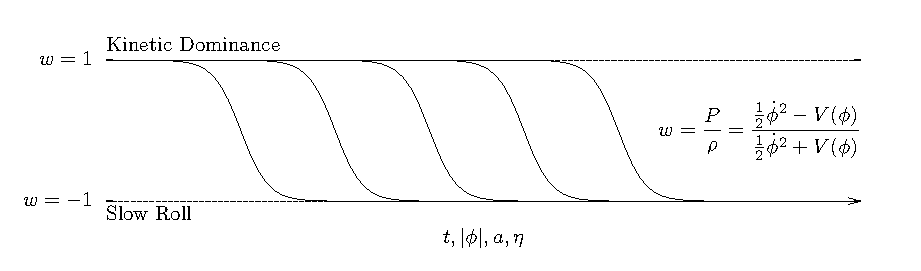
\includegraphics[width=\textwidth]{chapter_classical_perturbations/plots/w.eps}
  \caption{%
    Schematic of the equation of state parameter $w$ against cosmic
    evolution. The generic scenario entails beginning in a kinetically
    dominated phase with $w=1$ (i.e.\ $\dot{\phi}^2\gg V(\phi)$)
    before moving to the typical slow roll attractor solution with
    $w=-1$ (i.e.\ $\dot{\phi}^2 \ll V(\phi)$). We term the
    intermediate stage ``Fast roll''.\label{fig:w}
  }
\end{figure}
%%%%%%%%%%%%%%%%%%%%%%%%%%%%%%%%%%%%%%%%%%%%%%%%%%%%%%%%%%%%%%%%%%%%%%

This statement is rigorously true. However, the key question is how
physically relevant it is. The classical equations have two
opportunities to break down:
\begin{enumerate}
  \item At the Planck time $\tp$.
  \item If we move out of the linear perturbative approximation.
\end{enumerate}


\section{The Planck time $\tp$}
The Planck epoch occurs at the earliest times and is defined as the
regime in which we are certain we would need a quantum theory of
gravity. Effectively this occurs when:
\begin{equation}
  \rho = \frac{1}{2}\dot\phi^2 + V(\phi)  \sim \m^4
  \label{eqn:rhosim}
\end{equation}
If the universe exits the kinetically dominated solutions before the
Planck time, then kinetic dominance cannot be physically relevant. We
may use this to put bounds on $\phip$, or alternatively the total
number of $e$-folds of inflation.

If we are in the kinetically dominated phase with $\dot{\phi}^2\gg
V(\phi)$ then
\begin{equation}
              \rho \approx \frac{1}{2}\dot\phi^2= \frac{1\m^2}{3t^2} 
  \label{eqn:rhop}
\end{equation}
so $\rho\sim\m^4$ implies that $t\sim\tp=\m^{-1}$. Thus, in order for
kinetic dominance to be true at the Planck time we require that
\begin{equation}
  V(\phip) \ll \m^4
\end{equation}
For $\m^2\phi^2$ inflation, this amounts to requiring that $\phip^2\ll
\frac{\m^4}{m^2}$. In order to agree with CMB observations, we require
that $m\sim10^{-5}\m$, which amounts to requiring that 
\begin{equation}
 \phip^2 \ll 10^{10}\m^2 \nonumber.
 \label{eqn:phipbound}
\end{equation}

We may phrase this in terms of the total number of $e$-folds:
\begin{align}
  N_\mathrm{tot} 
  &=\int_{t_\mathrm{begin}}^{t_\mathrm{end}} H dt 
  =\int_{\phi_\mathrm{begin}}^{\phi_\mathrm{end}} 
       \frac{H}{\dot{\phi}}d\phi  &\text{($H=\dot{N}$)}
  \\
  &=\frac{1}{\m^2}\int_{\phi_\mathrm{begin}}^{\phi_\mathrm{end}}
     {\frac{V(\phi)}{V^\prime(\phi)}}d\phi &\text{Slow Roll.}
\end{align}
For $V\sim\phi^n$, this gives:
\begin{equation}
  N = \frac{\Delta (\phi^2) }{n\:\m^2}
\end{equation}
If we take our upper bound (\ref{eqn:phipbound}), and assume that the
end of inflation is somewhere near the base of the potential, we find
that: 
\begin{equation}
  N_\mathrm{tot}\ll 10^{10}.
\end{equation}
It is difficult to imagine how one could possibly constrain the total
number of $e$-folds observationally, unless the number was
sufficiently small so as to be observable directly in the CMB power
spectrum (for example in ``just enough inflation''). There are
theoretical limits, but these typically tend to be much, much larger
than this.

The typical argument (Linde) goes something like this:

\begin{enumerate}
  \item We should set initial conditions at the Planck time, when
    $\rho\sim\m^4$.
  \item There will be some partitioning between kinetic and potential
    energy at this moment.
  \item Given that we know nothing of the physics we should put
    uniform priors the amount of energy in the potential at this
    moment: $V(\phip)\in[0,\m^4]$.
  \item Therefore on average we expect equipartition between kinetic
    and potential energy at the Planck time
\end{enumerate}

From Linde's argument, the kinetically dominated regime is only present
after the Planck time for $V(\phip)$ at the very bottom end of the
prior range.

We can see this graphically in Figure~\ref{fig:cls:linde}

\ifdefined\lightweight{}
\else
\begin{figure}
  \centering
  \includegraphics[width=\textwidth]{chapter_classical_perturbations/plots/swirl.tikz}
  \includegraphics[width=\textwidth]{chapter_classical_perturbations/plots/true.tikz}
  \caption{Linde's initial conditions. These are phase-space plots of the evolution of $(\phi,\dot{\phi})$, plotted for a chaotic inflationary potential $V(\phi) = \frac{1}{2}m^2 \phi^2$. The upper plot has $m=0.5$. The outer circle is the Planck time $\tp$ when $\rho=\m^4$. One can see that each path through phase space is generically drawn to the slow roll attractor solutions in the center of the plot. The lines are plotted so that they have a uniform spacing of kinetic energy at the Planck time. As you can see, only a very small number of the solutions satisfy kinetic dominance at any point. \\
  The upper plot is somewhat misleading, since it has an artificially high value of $m$. When the value of $m$ is lowered to $0.1\m$, as in the lower plot, then the slow roll phase is a much stronger attractor solution, and generates a sustained slow-roll accelerated expansion.\label{fig:cls:linde}}
\end{figure}

\begin{figure}
  \centering
  \includegraphics[width=\textwidth]{chapter_classical_perturbations/plots/swirl_alt.tikz}
  \includegraphics[width=\textwidth]{chapter_classical_perturbations/plots/true_alt.tikz}
  \caption{Post-inflationary initial conditions}
\end{figure}
\fi




\section{The linear approximation}
To first order, the $i$-$j$, $i$-$0$ and $0$-$0$ Einstein equations read:
\begin{align}
  \Phi &= \Psi 
  \label{eqn:clp:Eij} \\
  0 &= -\dot{\phi}\:\delta\phi  + 2 H \Phi + 2 \dot{\Phi} 
  \label{eqn:clp:Ei0}\\
  0 &= \left(6H^2-\dot{\phi}^2 + 2\frac{k^2}{a^2}\right)\Phi  + \left( -3H\dot{\phi} - \ddot{\phi} \right)\delta\phi + \dot{\phi}\delta\dot{\phi} +  6 H \dot{\Phi},
  \label{eqn:clp:E00}
\end{align}
where we have absorbed the explicit potential dependence into $\ddot{\phi}$ terms. 
One may rearrange these to gain second order equations in $\Phi$ or $\mathcal{R}$:
\begin{align}
  0 &= \ddot{\Phi} + \left( H - 2 \frac{\ddot{\phi}}{\dot{\phi}} \right) \dot{\Phi} + \left( \frac{k^2}{a^2}-\frac{1}{\m^2}\dot{\phi}^2 - 2\frac{\ddot{\phi}}{\dot{\phi}}H \right)\Phi, \\
  0 &= \ddot{\mathcal{R}} + \left( \frac{\dot{\phi}^2}{\m^2H} + 3H + 2\frac{\ddot{\phi}}{\dot{\phi}} \right)\dot{\mathcal{R}} + \frac{k^2}{a^2}\mathcal{R}, \qquad \mathcal{R} = \Psi - \frac{H}{\dot{\phi}}\delta\phi
\end{align}
There is of course also a second order equation purely in $\delta\phi$, but this is particularly unappetising, and given that we have an explicit solution for it in~\eqref{eqn:clp:Ei0}, we shall not state it here.
Technically, these equations are derived in the Newtonian gauge ($E=B=0$), but since everything here is manifestly gauge invariant one may interpret all of the above equations as the relations in the equivalent gauge invariant variables.

If we apply the kinetically dominated solutions to the background variables, the perturbed variables are soluble with Bessel functions. There are two constants of integration, in the above equations. Examining the limit as $t\to 0$, one finds that all of the variables have a ``freezing mode'' and a ``growing mode'', i.e:
\begin{equation}
  \Phi\sim \delta\phi \sim \mathcal{R} = A + B t^{-4/3} \qquad \text{as } t\rightarrow 0,
\end{equation}
where $A$ and $B$ are constants of integration.
The growing mode in $\log t$ technically violates the initial perturbative assumption. It may be the case that a more sophisticated expansion out of the big bang is required.

We may rearrange equations~\eqref{eqn:clp:Ei0} and~\eqref{eqn:clp:E00} as:
\begin{align}
  \frac{d}{dt}
  \left(
  \begin{array}{c}
    \delta \phi \\
    \Phi
  \end{array}
  \right)
  =
  \left(%
  \begin{array}{cc}
    \frac{\ddot{\phi}}{\dot{\phi}} & \frac{1}{\dot{\phi}}\left( \dot{\phi}^2 - 2\frac{k^2}{a^2} \right) \\
    \frac{1}{2}\dot{\phi} & -H 
  \end{array}
  \right)
  \left(%
  \begin{array}{c}
    \delta \phi \\
    \Phi
  \end{array}
  \right)
\end{align}


Is there an alternative variable which freezes out in the kinetically dominated phase? Yes, there must be. What is it? What is the best way to find out what it is? Is it gauge invariant?


\section{Working}
In the Newtonian gauge we have:
\begin{align}
  \frac{d}{dt}
  \left(
  \begin{array}{c}
    \delta \phi \\
    \Phi
  \end{array}
  \right)
  &=
  \left(%
  \begin{array}{cc}
    \frac{\ddot{\phi}}{\dot{\phi}} & \frac{1}{\dot{\phi}}\left( \dot{\phi}^2 - 2\frac{k^2}{a^2} \right) \\
    \frac{1}{2}\dot{\phi} & -H 
  \end{array}
  \right)
  \left(%
  \begin{array}{c}
    \delta \phi \\
    \Phi
  \end{array}
  \right)\label{eqn:cls:fstodr}
  \\
  \Psi{} &= \Phi{}
\end{align}

Now, some gauge invariant variables are:
\begin{align}
  \mathcal{R} &= \Psi + \frac{H}{\dot{\phi}}\delta\phi \\
  \mathcal{S} &= \Phi + \frac{\d{}}{\d{t}}\left(\frac{\Psi}{H}\right)
\end{align}
We can re-phrase the dynamical equations in terms of these, giving us a set of gauge invariant ones. Eliminating first derivatives of $\Phi$ using~\eqref{eqn:cls:fstodr}, one finds:
\begin{equation}
  \left(
  \begin{array}{c}
    \mathcal{R} \\
    \mathcal{S}
  \end{array}
  \right)
  =
  \left(%
  \begin{array}{cc}
    \frac{H}{\dot{\phi}} & 1 \\
    \frac{\dot{\phi}}{2H} & \frac{\dot{\phi}^2}{2H^2}
  \end{array}
  \right)
  \left(%
  \begin{array}{c}
    \delta \phi \\
    \Phi
  \end{array}
  \right).
\end{equation}

This is singular\ldots

\pagebreak

Inverting the above relation yields:
\begin{equation}
  \left(%
  \begin{array}{c}
    \delta \phi \\
    \Phi
  \end{array}
  \right)
  =
  \left(%
  \begin{array}{cc}
    -\frac{\dot{\phi}}{2H} & \frac{H}{\dot{\phi}} \\
    \frac{1}{2} & \frac{H^2}{\dot{\phi}^2}
  \end{array}
  \right)
  \left(%
  \begin{array}{c}
    \mathcal{R} \\
    \mathcal{S}
  \end{array}
  \right).
\end{equation}
Substituting this into~\eqref{eqn:cls:fstodr} yields:
\begin{align}
  \frac{d}{dt}
  \left(%
  \begin{array}{c}
    \mathcal{R} \\
    \mathcal{S}
  \end{array}
  \right)
  &=
  \left(%
  \begin{array}{cc}
    & \\
    &
  \end{array}
  \right)
  \left(%
  \begin{array}{c}
    \mathcal{R} \\
    \mathcal{S}
  \end{array}
  \right).
\end{align}
